\documentclass[12pt,a4paper]{article}
%\usepackage{fontspec, xunicode, xltxtra}  
%\setmainfont{Hiragino Sans GB}  
\usepackage{xeCJK}
%\setCJKmainfont[BoldFont=STZhongsong, ItalicFont=STKaiti]{STSong}
%\setCJKsansfont[BoldFont=STHeiti]{STXihei}
%\setCJKmonofont{STFangsong}

%使用Xelatex编译

% 设置页面
%==================================================
\linespread{2} %行距
% \usepackage[top=1in,bottom=1in,left=1.25in,right=1.25in]{geometry}
% \headsep=2cm
% \textwidth=16cm \textheight=24.2cm
%==================================================

% 其它需要使用的宏包
%==================================================
\usepackage[colorlinks,linkcolor=blue,anchorcolor=red,citecolor=green,urlcolor=blue]{hyperref} 
\usepackage{tabularx}
\usepackage{authblk}         % 作者信息
\usepackage{algorithm}     % 算法排版
\usepackage{amsmath}     % 数学符号与公式
\usepackage{amsfonts}     % 数学符号与字体
\usepackage{mathrsfs}      % 花体
\usepackage{amssymb}


\usepackage{graphics}
\usepackage{color}
\usepackage{fancyhdr}       % 设置页眉页脚
\usepackage{fancyvrb}       % 抄录环境
\usepackage{float}              % 管理浮动体
\usepackage{geometry}     % 定制页面格式
\usepackage{hyperref}       % 为PDF文档创建超链接
\usepackage{lineno}          % 生成行号
\usepackage{listings}        % 插入程序源代码
\usepackage{multicol}       % 多栏排版
%\usepackage{natbib}         % 管理文献引用
\usepackage{rotating}       % 旋转文字,图形,表格
\usepackage{subfigure}    % 排版子图形
\usepackage{titlesec}       % 改变章节标题格式
\usepackage{moresize}   % 更多字体大小
\usepackage{anysize}
\usepackage{indentfirst}  % 首段缩进
\usepackage{booktabs}   % 使用\multicolumn
\usepackage{multirow}    % 使用\multirow
\usepackage{graphicx} 
\usepackage{wrapfig}
\usepackage{xcolor}
\usepackage{titlesec}     % 改变标题样式
\usepackage{enumitem}

\newcommand{\myvec}[1]%
   {\stackrel{\raisebox{-2pt}[0pt][0pt]{\small$\rightharpoonup$}}{#1}}  %矢量符号
\renewcommand{\vec}[1]{\boldsymbol{#1}}
\newcommand{\me}{\mathrm{e}}
\newcommand{\mi}{\mathrm{i}}
\newcommand{\dif}{\mathrm{d}}
\newcommand{\tabincell}[2]{\begin{tabular}{@{}#1@{}}#2\end{tabular}}

\def\kpc{{\rm kpc}}
\def\km{{\rm km}}
\def\cm{{\rm cm}}
\def\TeV{{\rm TeV}}
\def\GeV{{\rm GeV}}
\def\MeV{{\rm MeV}}
\def\GV{{\rm GV}}
\def\MV{{\rm MV}}
\def\yr{{\rm yr}}
\def\s{{\rm s}}
\def\ns{{\rm ns}}
\def\GHz{{\rm GHz}}
\def\muGs{{\rm \mu Gs}}
\def\arcsec{{\rm arcsec}}
\def\K{{\rm K}}
\def\microK{\mu{\rm K}}
\def\sr{{\rm sr}}
\newcolumntype{p}{D{,}{\pm}{-1}}

\renewcommand{\figurename}{Fig.}
\renewcommand{\tablename}{Tab.}

\renewcommand{\arraystretch}{1.5}

\setlength{\parindent}{0pt}  %取消每段开头的空格

\title{质点碰撞}
\author{}
\date{\today}
\begin{document}

\maketitle

微观粒子的碰撞又称\textcolor{red}{散射};

两物体的碰撞,通常发生在比较短暂的时间内,外界对这两物体或无作用,或虽有力的作用,但只要作用力是有限的,其冲量就可以忽略,体系的动量就是守恒的;
\section{正碰}
碰撞前两物体速度$\vec{u}_1$、$\vec{u}_2$均沿两球中心连线;

碰后两球的速度$\vec{v}_1$、$\vec{v}_2$和$\vec{u}_1$、$\vec{u}_2$在同一直线上;

取两球中心连线为坐标轴,以$\vec{u}_1$的方向为轴的正方向,设两球的质量分别为$m_1$、$m_2$,
\begin{equation}
m_1 u_1 + m_2 u_2 = m_1 v_1 + m_2 v_2
\end{equation}

\subsection{弹性碰撞}
在碰撞过程中没有机械能损失的碰撞;
\begin{equation}
\frac{1}{2} m_1 u_1^2 +\frac{1}{2} m_2 u_2^2 = \frac{1}{2} m_1 v_1^2 +\frac{1}{2} m_2 v_2^2
\end{equation}

\begin{eqnarray}
\nonumber v_1 &=& \frac{m_1 -m_2}{m_1 +m_2} u_1 +\frac{2m_2}{m_1 +m_2} u_2 ~,\\
v_2 &=& \frac{2m_1}{m_1 +m_2} u_1 -\frac{m_1 -m_2}{m_1 +m_2} u_2 ~,
\end{eqnarray}

1. $m_1 = m_2$

$v_1 = u_2$,$v_2 = u_1$,即\textcolor{red}{碰后两球速度互相变换};

2. $u_2 = 0$,即\textcolor{red}{受碰球原先静止};

\begin{eqnarray}
\nonumber v_1 &=& \frac{m_1 -m_2}{m_1 +m_2} u_1 ~, \\
v_2 &=& \frac{2m_1}{m_1 +m_2} u_1 ~,
\end{eqnarray}
若\textcolor{red}{$m_1 \ll m_2$},则$v_1 = -u_1$,$v_2 \approx 0$,即碰后,\textcolor{red}{大球几乎仍保持静止},\textcolor{red}{小球以相等的速率返回};

若\textcolor{red}{$m_1 = m_2$},则$v_1 = 0$,$v_2 = u_1$,即碰后,两球运动速度交换;

若\textcolor{red}{$m_1 \gg m_2$},则$v_1 \approx u_1$,$v_2 \approx 2u_1$,即\textcolor{red}{大球几乎以原来速度继续前进},\textcolor{red}{而小球以两倍于大球的速度前进};

$m_2$所得到的动能$\Delta E_k$与碰前$m_1$的动能$E_{k1}$之比:
\begin{eqnarray}
\nonumber \frac{\Delta E_k}{E_{k1}} &=& \frac{4m_1 m_2}{(m_1 +m_2)^2} ~, \\
&=& \frac{4m_1/m_2}{(1+m_1/m_2)^2}
\end{eqnarray}
$m_1$与$m_2$越接近,$m_2$获得的能量越多;


\cite{benacquista2018classical} The simplest form of a collision is the rebounding of a low-mass particle off of an infinitely massive, immovable object such as a wall or floor. \textcolor{yellow}{The momentum is not conserved}, and the change in momentum of the particle is caused by the impulse delivered by the normal force of the wall or floor during the collision. If the initial kinetic energy of the particle is conserved and not dissipated to other forms of energy such as heat or sound, then the collision is \textcolor{red}{\bf elastic}. For such a collision, the magnitude of the momentum of the particle is constant, but the direction changes. Since the impulse is normal to the surface, the angle of reflection is equal to the angle of incidence as measured with respect to the normal.

The collision is said to be \textcolor{red}{\bf inelastic} if some of the kinetic energy is lost to other forms of energy during the collision. The loss of kinetic energy can be described phenomenologically by the \textcolor{red}{\bf coefficient of restitution}, which parameterizes the reduction in rebound velocity. The symbol $e$ or $\eta$ is often used for the coefficient of restitution. In the case of an object colliding normal to a surface, the fraction of kinetic energy that is retained
after the collision is related to the coefficient of restitution by
\begin{equation}
\eta^2 \equiv \dfrac{K_{\rm final}}{K_{\rm initial}}
\end{equation}
where $\eta$ runs from $0$ (perfectly inelastic) to $1$ (elastic). For an inelastic collision of a ball with the floor at an angle, there may be different coefficients of restitution for the normal and parallel components of the velocity. Thus, the angle of incidence need not equal the angle of reflection for inelastic collisions.


\subsubsection{The Hard Sphere}
\cite{benacquista2018classical} Consider the scattering off of a hard sphere of radius $a$ located at the origin. We have the incident particle come in from the $-z$ direction. The incoming direction of the particle must be offset from the $z$-axis by a distance less than $a$ in order to collide with the sphere. This offset is known as the \textcolor{red}{\bf impact parameter} and is usually denoted by $b$. After the collision, the particle will go off on a straight trajectory deflected by an angle $\theta$ with respect to the incoming trajectory. This angle corresponds to the polar angle $\theta$ in spherical coordinates. At the point of impact, the particle reaches $r_{\rm min}$, its distance of closest approach. For the hard sphere, $r_{\rm min} = a$. The point of impact can also be described by the polar angle $\phi_{m}$. (The momentum is not conserved.)

We don't consider rotating particles here, so the scattering force is strictly the normal force between the particle and the sphere, and it is directed radially outward. The impulse of this force is such that it simply reverses the direction of the component of the particle’s momentum that is normal to the surface of the sphere at the point of contact. From Fig. \ref{fig:hard_sphere}, we see that we can write the initial momentum as $\vec{p}_i = p \vec{\hat{z}}$. The component of momentum normal to the surface is $(\vec{p}_i \cdot \vec{\hat{n}}) \vec{\hat{n}}$ with $ \vec{\hat{n}} = \sin \phi_m \vec{\hat{x}} + \cos \phi_m \vec{\hat{z}}$. The scattered momentum vector is 
\begin{equation}
\vec{p}_r = \vec{p}_i +\Delta \vec{p} ~,
\end{equation}
where
\begin{equation}
\Delta \vec{p} = \Delta p \vec{\hat{n}} ~, ~~~ \Delta p = 2 |\vec{p}_i \cdot \vec{\hat{n}}| = -2 p \cos \phi_m ~.
\end{equation}
Note that $\Delta p \geqslant 0$ because $\pi/2 \leqslant \phi_m \leqslant \pi$. The scattered momentum vector is
\begin{equation}
\vec{p}_r = -p (\sin 2\phi_m \vec{\hat{x} } + \cos 2 \phi_m \vec{\hat{z}}) ~.
\end{equation}
$\phi_i + \phi_m = \pi \Longrightarrow \phi_m = \pi - \phi_i$,
\begin{equation}
\sin 2\phi_m = -\sin 2\phi_i ~, \cos 2\phi_m = \cos 2\phi_i ~,
\end{equation}
\begin{equation}
\vec{p}_r = p (\sin 2\phi_i \vec{\hat{x}} - \cos 2 \phi_i \vec{\hat{z}} ) ~.
\end{equation}
Thus, $\phi_i = \phi_m$, and the scattering angle $\theta = \pi - 2\phi_i$. $b = a \sin \phi_i$, so
\begin{align}
\theta &= \pi - 2 \arcsin \left(\dfrac{b}{a} \right) ~, \\
b &= a \cos \left(\dfrac{\theta}{2} \right) ~.
\end{align}
There is no scattering if $b > a$. The \textcolor{red}{total cross section $\sigma_T$} for the interaction of the particle with the hard sphere is defined as the area covered by values of $b$ that result in a scattering interaction. For the case of the hard sphere, the total cross section for an interaction is simply its geometrical cross-sectional area
\begin{equation}
\color{red}  \bf \sigma_T = \pi a^2 ~.
\end{equation}

%===========================================================================================================================
\begin{figure*}
\centering
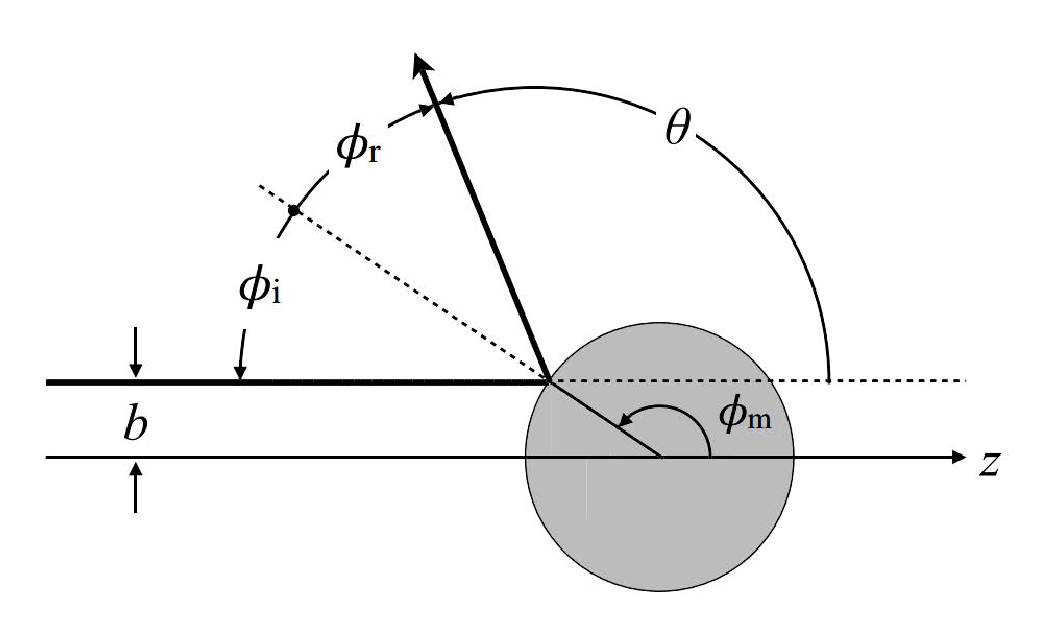
\includegraphics[height=6.cm, angle=0]{hard_sphere.eps}
\caption{The configuration for the scattering of a point particle off of a fixed hard sphere of radius $a$. The particle comes in from the left (from the $-z$ direction) with an impact parameter of $b$, and strikes the surface of the sphere at an angle of $\phi_i$ relative to the normal of the surface. The polar angle of the normal is the angle $\phi_m$, which describes the point of closest approach. After scattering, the particle leaves the sphere at an angle $\phi_r$ relative to the normal. The final trajectory is described by the polar angle $\theta$.
}
\label{fig:hard_sphere}
\end{figure*}
%===========================================================================================================================


\subsubsection{Differential Cross Section}
\cite{benacquista2018classical} 






\textcolor{orange}{要理解卢瑟福散射公式,就是要理解为什么通过计数散射出的粒子数来得到碰撞截面。首先研究硬球散射。假设一束流总共有$N$个粒子,入射面积为$A$,向球射来。假设入射粒子半径很小,可以忽略不计。当入射粒子的碰撞参数$b$大于硬球半径时,粒子不和硬球发生相互作用,其运动方向不发生改变,$\theta = \theta^\prime = 0$。当入射粒子的碰撞参数$b$小于硬球半径时,粒子与硬球发生完全弹性散射,其碰撞参数$b$和偏转角$\theta$的关系可以通过反射定律得到
\begin{align*}
\dfrac{b}{R} &= \sin \phi = \sin \dfrac{\pi -\theta}{2} = \cos \dfrac{\theta}{2} ~, \\
|\dif b| &= \dfrac{R}{2} \sin \dfrac{\theta}{2} \dif \theta
\end{align*}
$b |\dif b| \dif \phi$范围内的粒子散射到$\theta \rightarrow \theta +\dif \theta$以及$\phi \rightarrow \phi + \dif \phi$方向的粒子数为
\begin{align*}
\dif N = \dfrac{N}{A} b |\dif b| \dif \phi = \dfrac{N}{A} \dfrac{R^2}{2} \sin \dfrac{\theta}{2} \cos \dfrac{\theta}{2}  \dif \theta \dif \phi = \dfrac{N}{A} \dfrac{R^2}{4} \sin \theta \dif \theta \dif \phi = \dfrac{N}{A} \dfrac{R^2}{4} \dif \Omega
\end{align*}
对整个立体角积分,我们可以得到所有散射的粒子数
\begin{equation*}
\Delta N = \int \dfrac{N}{A} \dfrac{R^2}{4} \dif \Omega = \dfrac{N}{A} \pi R^2 ~.
\end{equation*}
将面积$A$乘以散射的粒子比例,也就是$\dfrac{\Delta N}{N}$,得到散射的截面$\sigma$,也就是
\begin{equation*}
\sigma = \pi R^2 ~.
\end{equation*}
散射到$\dif \Omega$立体角对应的截面,也就是面积$A$乘以散射到$\dif \Omega$的粒子比例,即$A\cdot \dfrac{\dif N}{N}$,称为微分散射截面,也就是
\begin{equation*}
A\cdot \dfrac{\dif N}{N \dif \Omega} = \dfrac{\dif \sigma}{\dif \Omega} = \dfrac{b |\dif b| \dif \phi}{\dif \Omega} ~, \rightarrow \dfrac{\dif \sigma}{\dif \Omega} \dif \Omega = b |\dif b| \dif \phi
\end{equation*}
对于硬球散射,微分散射截面就是
\begin{equation*}
\dfrac{\dif \sigma}{\dif \Omega} = \dfrac{R^2}{4} ~.
\end{equation*}
推广到卢瑟福散射,碰撞参数$b$与散射角的关系为库伦公式
\begin{equation*}
b = \dfrac{a}{2} \cot \dfrac{\theta}{2} ~, \\
|\dif b| = \dfrac{a}{4} \dfrac{\dif \theta}{\sin^2 \dfrac{\theta}{2} }
\end{equation*}
假设一束粒子流$N$,面积为$A$,打到薄膜上,薄膜的厚度为$t$,(单位体积内的原子核数)原子核数密度为$n$,微分散射截面为
\begin{align*}
b |\dif b| \dif \phi &= \dfrac{a^2}{8} \dfrac{\cos \dfrac{\theta}{2} \dif \theta}{\sin^3 \dfrac{\theta}{2} }  \dif \phi = \dfrac{a^2}{8} \dfrac{\cos \dfrac{\theta}{2} \sin \dfrac{\theta}{2} \dif \theta}{\sin^4 \dfrac{\theta}{2} }  \dif \phi = \dfrac{a^2}{16} \dfrac{ \sin  \theta \dif \theta \dif \phi}{\sin^4 \dfrac{\theta}{2} } ~, \\
\dfrac{\dif \sigma}{\dif \Omega} &= \dfrac{b |\dif b| \dif \phi}{\dif \Omega} = \dfrac{a^2}{16} \dfrac{1}{\sin^4 \dfrac{\theta}{2} } = \left( \dfrac{Z_1 Z_2 e^2}{4\pi \epsilon_0} \dfrac{1}{4 E} \right)^2 \dfrac{1}{\sin^4 \dfrac{\theta}{2} } ~.
\end{align*}
和之前的硬球碰撞不同,$N$个粒子打在一个硬球上,单位立体角散射的粒子数为$\dfrac{\Delta N}{\dif \Omega}$,这里是单位立体角散射的粒子数为$\dfrac{\Delta N}{\dif \Omega}$是薄膜上很多个原子核散射造成的,因此单个粒子的微分散射截面需要除以薄膜上总的散射的原子核,即$A n t$,因此为
\begin{equation}
A\dfrac{\dif N}{N\dif \Omega} \dfrac{1}{A nt} = \dfrac{\dif N}{ntN\dif \Omega}  = \dfrac{\dif \sigma}{\dif \Omega} = \left( \dfrac{Z_1 Z_2 e^2}{4\pi \epsilon_0} \dfrac{1}{4 E} \right)^2 \dfrac{1}{\sin^4 \dfrac{\theta}{2} } ~.
\end{equation}
可以看出散射的粒子数和入射流的面积$A$无关,也就是说所有粒子$N$均匀地先后打在一个靶核子上和一次打在许多靶核子上,最后散射到立体角$\dif \Omega$内的粒子数是一样的。
}


\subsection{非弹性碰撞}
碰撞过程中形变不能完全消失,机械能不守恒,其中一部分转化为内能;

\subsubsection{完全非弹性碰撞}
设形变是范性的,一旦发生形变就永久保持,完全不能消失;只有压缩阶段,没有恢复阶段,两球达到相同速度后即停止,尔后两球以共同速度前进;

动量仍然守恒
\begin{equation}
m_1 u_1 + m_2 u_2 = (m_1 +m_2) v
\end{equation}
但机械能不再守恒,损失的机械能为
\begin{eqnarray}
\nonumber \Delta E &=& \frac{1}{2} m_1 u_1^2 +\frac{1}{2} m_2 u_2^2 -\frac{1}{2}(m_1 +m_2)v^2 ~,\\
&=& \frac{1}{2} \frac{m_1 m_2(u_1-u_2)^2}{(m_1 +m_2)}
\end{eqnarray}

当$u_2 = 0$时,
\begin{eqnarray}
\Delta E = \frac{1}{2} m_1 u_1^2 \frac{m_2}{m_1 +m_2} = E_{k1} \frac{m_2}{m_1 +m_2}
\end{eqnarray}
从而
\begin{equation}
\frac{\Delta E_k}{E_{k1}} = \frac{1}{1+m_1/m_2}
\end{equation}
为了在碰撞中,获得大的激发能或电离能,要求撞击粒子原来的能量大,且撞击粒子与被撞击粒子相比质量必须要小;

撞击粒子的动能不可能完全转化为激发能或电离能,因为在碰撞前后,质心的速度不变,与质心相联系的那部分动能即质心动能不可能转变成其他形式的能量;只有相当于质心的动能,才可能转变为其他形式的能量,称为\textcolor{red}{资用能};使质心动能尽量小;

\subsubsection{一般非弹性碰撞}
定义\textcolor{red}{恢复系数}:
\begin{equation}
e = \frac{v_2 -v_1}{u_1 -u_2}
\end{equation}
弹性碰撞中,
\begin{equation}
\frac{v_2 -v_1}{u_1 -u_2} = 1
\end{equation}
完全非弹性碰撞中,
\begin{equation}
\frac{v_2 -v_1}{u_1 -u_2} = 0
\end{equation}
恢复系数只与两球的质料有关,与碰前速度无关;

对一般非弹性碰撞,
\begin{equation}
0 < e < 1
\end{equation}

\begin{eqnarray}
\nonumber v_1 = \frac{m_1 -em_2}{m_1 +m_2}u_1 +\frac{(1+e)m_2}{m_1 +m_2} u_2 ~, \\
v_2 = \frac{(1+e)m_1}{m_1 +m_2} u_1 - \frac{em_1 -m_2}{m_1 +m_2}u_2 ~,
\end{eqnarray}

碰撞中损失的机械能为
\begin{equation}
\Delta E = \frac{1}{2}(1-e^2) \frac{m_1m_2}{m_1+m_2} (u_1 -u_2)^2
\end{equation}


\section{斜碰}
碰撞前两球的速度$\vec{u}_1$、$\vec{u}_2$不在两球中心连线上;一般情况,斜碰为三维问题,碰撞后的速度$\vec{v}_1$、$\vec{v}_2$不一定在$\vec{u}_1$、$\vec{u}_2$组成的平面上;

设弹性碰撞前一个小球处在静止状态,即$\vec{u}_2 = 0$,
\begin{eqnarray}
\nonumber m_1 \vec{u}_1 &=& m_1 \vec{v}_1 +  m_2 \vec{v}_2 ~,\\
\frac{1}{2} m_1 u_1^2 &=& \frac{1}{2} m_1 v_1^2 +\frac{1}{2} m_2 v_2^2 ~,
\end{eqnarray}
取$\vec{u}_1$方向为$x$轴,碰撞所在面为$x-y$面,
\begin{eqnarray}
m_1 u_1 &=& m_1 v_1 \cos \theta_1 +m_2 v_2 \cos \theta_2 ~, \\
0 &=& m_1 v_1 \sin \theta_1 -m_2 v_2 \sin \theta_2 ~, 
\end{eqnarray}
$\theta_1$、$\theta_2$称为散射角;

碰撞结果与碰前两小球中心在$y$方向的距离$b$有关,$b$称为\textcolor{red}{碰撞参数};$b = 0$时为正碰;

\section{碰撞与质心坐标系}
碰撞过程中,质心系仍是惯性系;

设$\vec{u}_2 = 0$,

\subsection{正碰}
\begin{equation}
v_C = \frac{m_1}{m_1 +m_2} u_1 ~,
\end{equation}
质心系中,碰前两球的速度为
\begin{eqnarray}
\nonumber u_1^{\prime} &=& u_1 -v_C = \frac{m_2}{m_1+m_2} u_1 ~, \\
u_2^{\prime} &=& u_2 -v_C = -\frac{m_1}{m_1 +m_2} u_1 ~, 
\end{eqnarray}
从而
\begin{equation}
m_1 u_1^{\prime} + m_2 u_2^{\prime} = 0
\end{equation}
即质心系中,体系的动量为$0$,

碰后,
\begin{equation}
m_1 v_1^{\prime} + m_2 v_2^{\prime} = 0
\end{equation}
质心系中碰撞前后体系动能仍相等,
\begin{eqnarray}
\nonumber v_1^{\prime} &=& -u_1^{\prime}  ~, \\
v_2^{\prime}  &=& -u_2^{\prime}  ~,
\end{eqnarray}
\textcolor{red}{在质心系中,粒子的速率在碰撞前后保持不变,但粒子速度反向};

回到实验室坐标系:
\begin{eqnarray}
v_1 &=& v_1^{\prime}  +v_C = \frac{m_1-m_2}{m_1+m_2} u_1 ~, \\
v_2 &=& v_2^{\prime}  +v_C =  \frac{2m_1}{m_1+m_2} u_1 ~, 
\end{eqnarray}

\subsection{斜碰}
质心速度
\begin{equation}
\vec{v}_C = \frac{m_1}{m_1 +m_2} \vec{u}_1
\end{equation}
质心系中,两质点碰前速度
\begin{eqnarray}
\nonumber \vec{u}_1^{\prime} &=& \vec{u}_1 -\vec{v}_C = \frac{m_2}{m_1+m_2} \vec{u}_1 ~, \\
 \vec{u}_2^{\prime} &=& \vec{u}_2 -\vec{v}_C = -\frac{m_1}{m_1+m_2} \vec{u}_1 ~,
\end{eqnarray}
碰撞前后,质心系中体系的动量为$0$,
\begin{equation}
m_1 \vec{u}_1^{\prime} + m_2 \vec{u}_2^{\prime} = m_1 \vec{v}_1^{\prime} + m_2 \vec{v}_2^{\prime} = 0
\end{equation}
\textcolor{red}{$\vec{v}_1^{\prime}$和$\vec{v}_2^{\prime}$仍在一直线上};且碰撞前后体系动能相等,
\begin{equation}
|\vec{v}^{\prime}_1| = |\vec{u}^{\prime}_1| ~, |\vec{v}^{\prime}_2| = |\vec{u}^{\prime}_2|
\end{equation}
质心系中,二粒子碰撞后,速度只改变方向,不改变大小,碰后两速度仍在一直线上,但直线的方位改变了;用粒子入射方向和出射方向的夹角$\Theta$表示粒子运动方向改变的程度,其值在$0 \sim \pi$之间,与碰撞参量有关;

回到实验室坐标系,
\begin{eqnarray}
\nonumber \vec{v}_1 &=& \vec{v}_1^{\prime}  +\vec{v}_C  ~, \\
\vec{v}_2 &=& \vec{v}_2^{\prime}  +\vec{v}_C  ~, 
\end{eqnarray}
由于
\begin{eqnarray}
\nonumber |\vec{v}^{\prime}_1| &=& |\vec{u}^{\prime}_1| = \frac{m_2}{m_1 +m_2}u_1 ~, \\ 
\nonumber |\vec{v}^{\prime}_2| &=& |\vec{u}^{\prime}_2| = \frac{m_1}{m_1+m_2} u_1 ~, \\
 |\vec{v}_C| &=& |\vec{u}^{\prime}_2| = \frac{m_1}{m_1+m_2} u_1 ~, 
\end{eqnarray}
当\textcolor{red}{$m_1 < m_2$}时,
\begin{equation}
|\vec{v}_C| < |\vec{v}_1^{\prime}| ~,
\end{equation}
$m_1$的散射角$\theta_1$取\textcolor{red}{$0 \sim \pi$};
当\textcolor{red}{$m_1 > m_2$}时,
\begin{equation}
|\vec{v}_C| > |\vec{v}_1^{\prime}| ~,
\end{equation}
$m_1$的散射角$\theta_1$\textcolor{red}{不可能大于}
\begin{equation}
\theta_{1 \text{max}} = \text{arcsin} \frac{m_2}{m_1} ~;
\end{equation}



\section{Compton散射}
\begin{eqnarray}
\nonumber E_{\lambda} + E_0 &=& E_{\lambda^{\prime}} +E ~, \\
\vec{p}_{\lambda} &=& \vec{p}_{\lambda^{\prime}} +\vec{p}
\end{eqnarray}
$\vec{p}_{\lambda}$和$\vec{p}_{\lambda}^{\prime}$分别表示光子碰撞前后的动量;且
\begin{eqnarray}
\nonumber E_{\lambda} &=& h\nu ~, \\
\nonumber E_0 &=& m_e c^2 ~, \\
\nonumber E &=& \gamma m_{e} c^2 ~, \\
E^2 &=& E_0^2 +p^2c^2 ~, 
\end{eqnarray}
平方后可得
\begin{equation}
p_{\lambda}^2 +p_{\lambda^{\prime}}^2 -2 p_{\lambda} p_{\lambda^{\prime}} \cos \theta = p^2
\end{equation}
\textcolor{red}{Compton散射公式}
\begin{equation}
\lambda^{\prime} -\lambda = \Delta \lambda = \frac{h}{m_e c} (1-\cos \theta)
\end{equation}
散射光子的能量
\begin{equation}
h\nu^{\prime} = \frac{h\nu}{1+\kappa (1-\cos \theta)} ~, ~\kappa = \frac{h\nu}{m_e c^2} ~, 
\end{equation}
反冲电子动能
\begin{equation}
E_k = h\nu -h\nu^{\prime} = h\nu \frac{\kappa(1-\cos \theta)}{1+\kappa (1-\cos \theta)}
\end{equation}
Compton散射引起的最大位移($\theta = \pi$)
\begin{equation}
\Delta \lambda = \frac{2h}{m_e c}  = 0.0049 ~~\text{nm}
\end{equation}
反冲电子的最大动能
\begin{equation}
E_{k, \text{max}} = h\nu \frac{2\kappa}{1+2\kappa} ~,
\end{equation}
相应光子的最小能量
\begin{equation}
E_{\lambda^{\prime}} = (h\nu^{\prime})_{\text{min}} = \frac{h\nu}{1+2\kappa} ~,
\end{equation}
电子的Compton波长
\begin{equation}
\lambda = \frac{hc}{m_e c^2} = \frac{1.24 ~\text{nm}\cdot \text{keV}}{511 ~\text{keV}} = 0.002426 ~\text{nm} ~,
\end{equation}
经典电子半径
\begin{equation}
m_e c^2 = \frac{e^2}{4\pi \epsilon_0 r_e} ~, \Longrightarrow r_e = \frac{e^2}{4\pi \epsilon_0 m_e c^2} \approx 2.8 ~\text{fm} ~,
\end{equation}

















































%%%%%%%%%%%%%%%%%%%%%%%%%%%%%%%%%%%%%%%%%%%%%%%%%%%%%%%%%%%%%%%%%%%%%%
\bibliographystyle{unsrt_update}
\bibliography{ref}
%%%%%%%%%%%%%%%%%%%%%%%%%%%%%%%%%%%%%%%%%%%%%%%%%%%%%%%%%%%%%%%%%%%%%%


\end{document}